\textbf{Pour cette première partie, aucune justification n'est demandée et une seule réponse est possible par question. Pour chaque question, reportez son numéro sur votre copie et indiquez votre réponse.}

Une réponse fausse ou l'absence de réponse n'enlève aucun point.

\subsection*{Question 1}
	On range les valeurs dans l'ordre croissant :  \np[°C]{-1}; \np[°C]{0}; \np[°C]{1}; \np[°C]{3}; \np[°C]{7}.

	La médiane est la valeur qui est au milieu de la série, {c'est \np[°C]{1}.}

\subsection*{Question 2}
	\begin{minipage}[t]{0.4\linewidth}
		C'est le {motif n°8} qui est l'image du motif n°4 par cette translation.
	\end{minipage}
	\hfill~
	\begin{tikzpicture}[baseline={(current bounding box.center)}]
		\draw[->, >=triangle 45,line width=1mm, red](3.2,0.8)--(4.7,-0.2);
		\draw[->, >=triangle 45,line width=1mm, blue](0.7,-0.2)--(2.2,-1.2);
		\foreach \n/\x/\y in{1/0/0,2/2/0,3/4/0,4/-0.5/-1,5/1.5/-1,6/3.5/-1,7/-1/-2,8/1/-2,9/3/-2}{\begin{scope}[shift={(\x,\y)},rotate=0]
				\draw[line width=0.3mm](0,0)--(1,0.5)--(2,0)--(2.5,1)--(1.5,1.5)--(0.5,1)--cycle;\draw(1,0.8)node[right]{n°\n};
		\end{scope}}
	\end{tikzpicture}\hfill~

\subsection*{Question 3}
	Il y a 8 boules dont 3 sont rouges, donc {{$P(\text{rouge})=\dfrac38=\np{0.375}$}}

\subsection*{Question 4}
	\begin{minipage}{0.45\linewidth}
	On utilise la formule apprise par c\oe{}ur \textbf{CAH}.

	{$\cos\left(\widehat{\text{LKJ}}\right)=\dfrac{\text{adjacent}}{\text{hypoténuse}}=\dfrac{\text{LK}}{\text{JK}}$}
	\end{minipage}
	\hfill~
	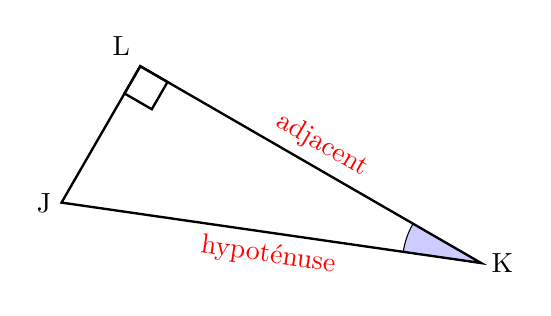
\begin{tikzpicture}[rotate=-30,baseline={(current bounding box.center)}]
		\draw[line width=0.3mm](0,0)rectangle(0.4,-0.4);
		\draw[fill=blue!20](5,0)--(4,0)arc(180:201.8:1)--cycle;
		\draw[line width=0.3mm](0,0)node[above left]{L}--(5,0)node[right]{K}node[midway, above, rotate=-30]{\textcolor{red}{adjacent}}--(0,-2)node[left]{J}node[midway, below, rotate=-8.2]{\textcolor{red}{hypoténuse}}--cycle;
	\end{tikzpicture}
	\hfill~

\subsection*{Question 5}
	{$\np{311200000}=\np{3.112}\times\np{100000000}$} \quad et \quad {$\np{100000000}=10^8$} (huit zéros),

	donc l'écriture scientifique de \np{311200000} est {$\np{3.112}\times10^8$}

\subsection*{Question 6}
	2~h~30~min c'est 2 heures plus la moitié d'une heure.

	Charlie a donc parcouru deux fois 40~km plus la moitié de 40~km :
	\quad $40 \times 2 + 40 \div 2 = 80 + 20 = 100$.

	Au total, {Charlie a fait 100~km.}

\subsection*{Question 7}
	{$5(x+1)=5\times x + 5\times 1 = 5x+5$}, donc la forme factorisée est {{$5(x+1)$}.}

\subsection*{Question 8}
	La diminution du prix est calculée par \quad
	\begin{tabular}{c|c|c}
		                & en \euro{} & en \% \\ \hline
		    baisse      &    $x$     &  10   \\ \hline
		valeur initiale &     80     &  100
	\end{tabular}

	{$x=80\times\dfrac{10}{100}$}, qu'il faut retrancher du prix initial, donc le calcul à effectuer est {	{$80-\dfrac{10}{100}\times80$}.}

\subsection*{Question 9}
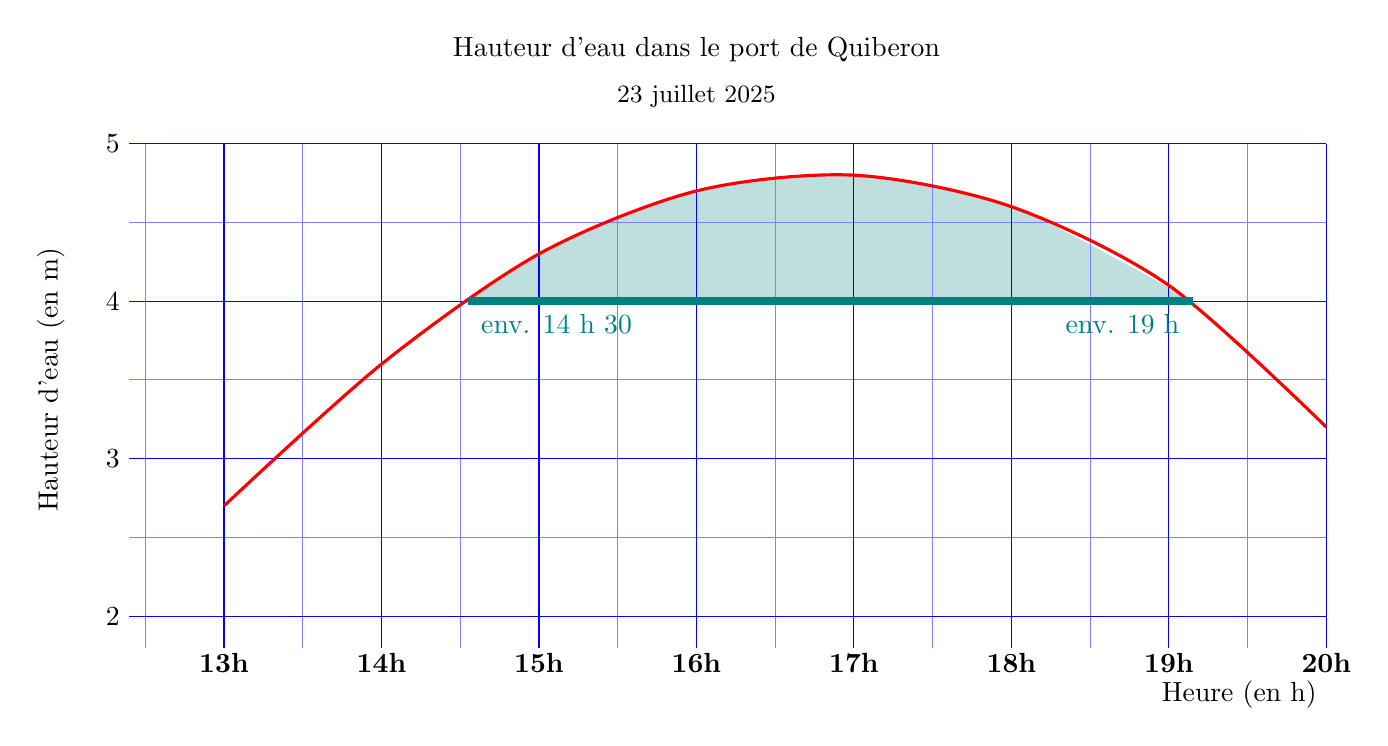
\begin{tikzpicture}[xscale=2,yscale=2]
	\fill[teal!25]plot[smooth]coordinates{(14.55,2)(15,2.3)(16,2.7)(17,2.8)(18,2.6)(19.15,2)}--cycle;
	\draw(11.9,1.5)node[rotate=90]{Hauteur d'eau (en m)};
	\draw(20,-0.5)node[left]{Heure (en h)};
	\draw(16,3.6)node{Hauteur d'eau dans le port de Quiberon};
	\draw(16,3.3)node{{\small 23 juillet 2025}};
	\draw[blue!50](12.4,-0.2)grid[step=0.5,dotted](20,3);
	\draw[blue](12.4,-0.2)grid[](20,3);
	\foreach \i in{13,14,...,20}{\draw(\i,-0.3)node{\textbf{\i h}};}
	\foreach \j in{0,1,2,3}{\pgfmathsetmacro{\leg}{int(\j+2)}\draw(12.4,\j)node[left]{\leg};}
	\draw[red, line width=0.4mm]plot[smooth]coordinates{(13,0.7)(14,1.6)(15,2.3)(16,2.7)(17,2.8)(18,2.6)(19,2.1)(20,1.2)};
	\draw[teal, line width=1mm](14.55,2)node[below right]{env. 14~h~30}--(19.15,2)node[below left]{env. 19~h};
\end{tikzpicture}

	Entre 14~h~30 à 19~h environ, le niveau a été plus élevé que 4~m, cela a donc duré {environ 4~h~30~min.}

\needspace{10\baselineskip}
